%!TEX program=xelatex

\documentclass[11pt]{ctexart}  
\usepackage[top=2cm, bottom=2cm, left=2cm, right=2cm]{geometry}  
\usepackage{algorithm}  
\usepackage{algorithmicx}  
\usepackage{algpseudocode}  
\usepackage{amsmath}  
\usepackage{graphicx}
\usepackage{amsmath}
\usepackage{amssymb}
\usepackage{enumerate}

\floatname{algorithm}{算法}
\renewcommand{\algorithmicrequire}{\textbf{输入:}}  
\renewcommand{\algorithmicensure}{\textbf{输出:}} 

\title{密码学实验报告5}
\author{张天辰 17377321}

\makeatletter
\newenvironment{breakablealgorithm}
  {% \begin{breakablealgorithm}
   \begin{center}
     \refstepcounter{algorithm}% New algorithm
     \hrule height.8pt depth0pt \kern2pt% \@fs@pre for \@fs@ruled
     \renewcommand{\caption}[2][\relax]{% Make a new \caption
       {\raggedright\textbf{\ALG@name~\thealgorithm} ##2\par}%
       \ifx\relax##1\relax % #1 is \relax
         \addcontentsline{loa}{algorithm}{\protect\numberline{\thealgorithm}##2}%
       \else % #1 is not \relax
         \addcontentsline{loa}{algorithm}{\protect\numberline{\thealgorithm}##1}%
       \fi
       \kern2pt\hrule\kern2pt
     }
  }{% \end{breakablealgorithm}
     \kern2pt\hrule\relax% \@fs@post for \@fs@ruled
   \end{center}
  }
\makeatother

\begin{document}
\maketitle{}



\section{AES算法}
\subsection{算法简介}
这里只讨论十轮AES。

加密算法输入为16字节的分组,组成一个$4 \times 4$的矩阵\textbf{$S$}。针对\textbf{$S$}有以下几种操作:

\begin{enumerate}[1]
    \item 字节代替。将\textbf{$S$}中的每个字节代替为S盒中的某个字节。代替规则为原始字节的前四位为行数,后四位为列数。考虑到算法实现的时间与空间的取舍,字节代替使用打表实现,因此算法毋需构造S盒。同理可以实现逆S盒用于解密。
    \item 行移位。将\textbf{$S$}中每一行分别循环左移0、1、2、3个字节,实现置换。类似地可以实现逆行移位用于解密。
    \item 列混淆。实际上可以写成如下的运算:
        \begin{equation}
            \textbf{S'} = {
            \begin{bmatrix}
                02 & 03 & 01 & 01 \\
                01 & 02 & 03 & 01 \\
                01 & 01 & 02 & 03 \\
                03 & 01 & 01 & 02
            \end{bmatrix}
            }\cdot \textbf{S}
        \end{equation}
        这里的所有运算都是基于$GF(2^8)$有限域上的运算,其中使用的8次不可约多项式为$x^8 + x^4 + x^3 + x + 1$。

        逆变换可以用相似的方法实现:
        \begin{equation}
            \textbf{S'} = {
            \begin{bmatrix}
                0E & 0B & 0D & 09 \\
                09 & 0E & 0B & 0D \\
                0D & 09 & 0E & 0B \\
                0B & 0D & 09 & 0E
            \end{bmatrix}
            }\cdot \textbf{S}
        \end{equation}
    \item 轮密钥加。每个字节与轮密钥中的对应字节异或。
    \end{enumerate}

密钥扩展算法中,将四个字节组成一个字,原始密钥生成初始四个字$w_0, w_1, w_2, w_3$。对$i \geqslant 4$,有:
\begin{equation}
    w_i = \left\{
    \begin{aligned}
        & w_{i-1} \oplus w_{i-4} \quad & 4 \nmid i \\
        & g(w_{i-1}) \oplus w{i-4} \quad & 4 \mid i
    \end{aligned}
    \right.
\end{equation}
每次取四个字组成轮密钥。

\subsection{算法实现}
算法都是类方法,所以可能没有参数。
\begin{enumerate}[1]
\item 密钥扩展算法
    \begin{enumerate}[(1)]
    \item $g$函数
    \begin{breakablealgorithm}  
    \caption{$g$函数}  
    \begin{algorithmic}[1] %每行显示行号  
        \Require 轮数$round$,待操作字$word$ 
        \Ensure 操作后字$tempWord$
        \Function {g}{$word, round$} 
            \State $tempWord \gets word[1:] + [word[0]]$
            \State $SBOX(tempWord)$
            \State $tempWord[0] \gets tempWord[0] \oplus RC[round]$
            \State \Return $tempWord$
        \EndFunction
    \end{algorithmic}  
    \end{breakablealgorithm}
    \item 密钥扩展
    \begin{breakablealgorithm}  
    \caption{密钥扩展}  
    \begin{algorithmic}[1] %每行显示行号  
        \Require 字列表$wordList$ 
        \Ensure 操作后字列表$wordList$
        \Function {generateKey}{$wordList$} 
            \For {$flag \in [4, 43]$}
                \If {$4|flag$}
                    \State $wordList[flag] \gets wordList[flag-1] \oplus$ \Call{g}{$wordList[flag-1], [flag/4]$}
                \Else
                    \State $wordList[flag] \gets wordList[flag-1] \oplus wordList[flag-1]$
                \EndIf
            \EndFor
        \EndFunction
    \end{algorithmic}  
    \end{breakablealgorithm}
    \end{enumerate}
\item AES加密部件算法
    \begin{enumerate}
        \item 字节代替。解密算法只需把算法中的SBOX替换成别的表即可。
        \begin{breakablealgorithm}  
        \caption{字节代替}  
        \begin{algorithmic}[1] %每行显示行号  
            \Function {substitute}{}
                \For {$i \in [0, 3]$}
                    \For {$j \in [0, 3]$}
                        \State $temp \gets S[i][j]$
                        \State $S[i][j] \gets SBOX[temp//16][temp \% 16]$
                    \EndFor
                \EndFor
            \EndFunction
        \end{algorithmic}  
        \end{breakablealgorithm}
        \item 行移位。解密算法只不过是左移改成右移,不再赘述。
        \begin{breakablealgorithm}  
        \caption{行移位}  
        \begin{algorithmic}[1] %每行显示行号  
            \Function {shiftRows}{}
                \State $S[1] \gets S[1][1:] + [S[1][0]]$
                \State $S[2] \gets S[2][2:] + S[2][:2]$
                \State $S[3] \gets [S[3][3]] + S[3][:3]$
            \EndFunction
        \end{algorithmic}  
        \end{breakablealgorithm}
        \item 列混淆。解密算法就是把mixColumnTable换成另一个表。算法中的$+$和$*$是有限域运算。
        \begin{breakablealgorithm}  
        \caption{列混淆}  
        \begin{algorithmic}[1] %每行显示行号  
            \Function {mixColumn}{}
                \State $temp \gets [[0 \times 4] \times 4]$
                \For {$i \in [0, 3]$}
                    \For {$j \in [0, 3]$}
                        \For {$k \in [0, 3]$}
                            \State $temp[i][j] \gets temp[i][j] + mixColumnTable[i][k] * S[k][j]$
                        \EndFor
                    \EndFor
                \EndFor
                \State $S \gets temp$
            \EndFunction
        \end{algorithmic}
        \end{breakablealgorithm}
        \item 轮密钥加,逆算法考虑到交换顺序,一并给出。算法中的$+$和$*$是有限域运算。
        \begin{breakablealgorithm}
        \caption{轮密钥加}  
        \begin{algorithmic}[1] %每行显示行号 
            \Require $key$ 
            \Function {addRoundKey}{$key$}
                \For {$i \in [0, 3]$}
                    \For {$j \in [0, 3]$}
                        \State $S[i][j] \gets S[i][j] \oplus key[i][j]$
                    \EndFor
                \EndFor
            \EndFunction
            \Function {revAddRoundKey}{$key$}
                \State $temp \gets [[0 \times 4] \times 4]$
                \For {$i \in [0, 3]$}
                    \For {$j \in [0, 3]$}
                        \For {$k \in [0, 3]$}
                            \State $temp[i][j] \gets temp[i][j] + revMixColumnTable[i][k] * key[k][j]$
                        \EndFor
                    \EndFor
                \EndFor
                \For {$i \in [0, 3]$}
                    \For {$j \in [0, 3]$}
                        \State $S[i][j] \gets S[i][j] \oplus temp[i][j]$
                    \EndFor
                \EndFor
            \EndFunction
        \end{algorithmic}  
        \end{breakablealgorithm}
    \end{enumerate}
\item AES算法
    \begin{breakablealgorithm}
        \caption{AES}  
        \begin{algorithmic}[1] %每行显示行号 
            \Require $key$扩展列表,$plain$(加密)$cipher$(解密) 
            \Ensure $cipher$(加密),$plain$(解密)
            \Function {AES\_Encrypt}{$plain, key$}
                \State $state \gets plain \to$ matrix
                \For {$round \in [0, 10]$}
                    \If {$round == 0$}
                        \State $state.addRoundKey(key.getRoundKey(round))$
                    \Else
                        \State $state.substitute()$
                        \State $state.shiftRows()$
                        \If {$round \neq 10$}
                            \State $state.mixColumn()$
                        \EndIf
                        \State $state.addRoundKey(key.getRoundKey(round))$
                    \EndIf
                \EndFor
                \State \Return $cipher \gets state \to$ 十六进制字符串
            \EndFunction
            \Function {AES\_Decrypt}{$cipher, key$}
                \State $state \gets copher \to$ matrix
                \For {$round \in [10 \to 0]$}
                    \If {$round == 10$}
                        \State $state.addRoundKey(key.getRoundKey(round))$
                    \Else
                        \State $state.revSubstitute()$
                        \State $state.revShiftRows()$
                        \If {$round \neq 0$}
                            \State $state.revMixColumn()$
                            \State $state.revAddRoundKey(key.getRoundKey(round))$
                        \Else
                            $state.addRoundKey(key.getRoundKey(round))$
                        \EndIf
                    \EndIf
                \EndFor
                \State \Return $plain \gets state \to$ 十六进制字符串
            \EndFunction
        \end{algorithmic}  
        \end{breakablealgorithm}
\end{enumerate}
\subsection{测试样例}
这里只测试加密,解密测试可以从此后大批量加密文件的测试中得到正确性的验证。
\begin{figure}[htbp]
\centering
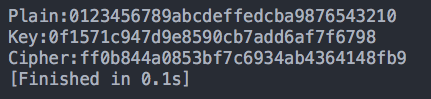
\includegraphics[height=2.97cm,width=12.93cm]{AES.png}
\caption{AES}
\label{aes}
\end{figure}
\section{AES工作模式}
\subsection{算法简介}
\begin{enumerate}[1]
\item 密文分组链接(CBC)
这种工作模式需要初始向量。将明文第一个分组加密后与初始向量异或得到第一组密文。对此后的每一组,将其加密后与前一组密文异或得到密文。这样的工作模式使得密文的每一个分组都与其之前的所有明文有关。解密时,将第一个密文分组解密后与初始向量异或,对此后每一组,将其解密后与前一组密文异或得到明文。

此外,这种工作模式需要对明文进行填充,以保证明文是整数个128bit分组。本方案采用PKCS5填充方式,即在最后一个分组为$x$个字节时:若$x<16$,则在$x$后填充$16-x$个字节,每个字节值为$16-x$;若$x=16$,则在$x$后填充16个字节,每个字节值为16。
\item 密文反馈模式(CFB)
这种工作模式也需要初始向量,但是不需要进行填充。使用移位寄存器,最初时为初始向量,并对其进行加密,只取第一个字节,然后与明文第一个字节异或得到密文第一个字节。对此后的每一组,将移位寄存器左移一个字节,并将上次加密得到的一个字节密文填充在最右侧,再进行加密即可。解密算法与加密算法几乎相同,差别存在于加密的移位寄存器填充的是加密得到的密文字节,而解密的移位寄存器填充的是解密前的密文字节。
\end{enumerate}
\subsection{算法实现}
算法都是类方法,所以可能没有参数。
\begin{enumerate}
    \item 密文分组链接CBC
        \begin{breakablealgorithm}  
        \caption{CBC}  
        \begin{algorithmic}[1] %每行显示行号  
            \Function {CBC\_Encrypt}{}
                \State $length \gets len(plain)$
                \State $cipher \gets []$
                \If {$16 | length$}
                    \State $plain.extend([16] * 16)$
                    \State $length += 16$
                \Else
                    \State $plain.extend([16 - length \%16] * (16-length\% 16)$
                    \State $length += 16-length\% 16$
                \EndIf
                \State $partEncrypt \gets AES()$
                \For {$i=0; i<length; i+=16$}
                    \State $partPlain \gets plain[i:i+16] \oplus initVector$
                    \State $partEncrypt.encrypt(partPlain, key)$
                    \State $cipher.append(partEncrypt.cipher)$
                    \State $initVector \gets partEncrypt.cipher$
                \EndFor
            \EndFunction
            \Function {CBC\_Decrypt}{}
                \State $plain \gets []$
                \State $partDecrypt \gets AES()$
                \For {$i=0; i<length; i+=16$}
                    \State $partDecrypt.decrypt(cipher[i:i+16], key)$
                    \State $partPlain \gets partDecrypt.plain \oplus initVector$
                    \State $plain.append(partPlain)$
                    \State $initVector \gets cipher[i:i+16]$
                \EndFor
                \State $paddle \gets plain[-1][-2:]$
                \State $plain[-1] \gets plain[-1][:-2*paddle]$
            \EndFunction
        \end{algorithmic}  
        \end{breakablealgorithm}
    \item 密文反馈模式CFB
        \begin{breakablealgorithm}  
        \caption{CFB}  
        \begin{algorithmic}[1] %每行显示行号  
            \Function {CFB}{$mode$}
                \State $shiftReg \gets initVector$
                \State $source \gets AES()$
                \State $targets \gets []$
                \For {$p \in sources$}
                    \State $source.encrypt(shiftReg, key)$
                    \State $target \gets source.cipher[:2] \oplus p$
                    \If {$mode == "ENCRYPT"$}
                        \State $shiftReg \gets shiftReg[2:] + target$
                    \Else 
                        \State $shiftReg \gets shiftReg[2:] + p$
                    \EndIf
                    \State $targets.append(target)$
                \EndFor
            \EndFunction
        \end{algorithmic}  
        \end{breakablealgorithm}
\end{enumerate}
\subsection{测试样例}
本方案实现了GUI界面。通过二进制读写文件,可以实现大小不太大的任意文件的加密。
\begin{figure}[htbp]
\centering
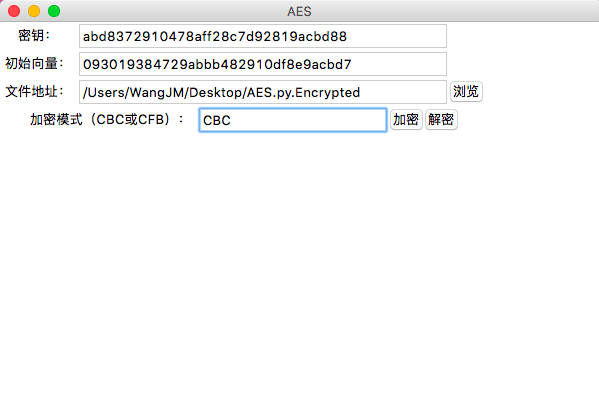
\includegraphics[height=8.40cm,width=11.98cm]{encrypt.png}
\caption{加密}
\label{encrypt}
\end{figure}
\begin{figure}[htbp]
\centering
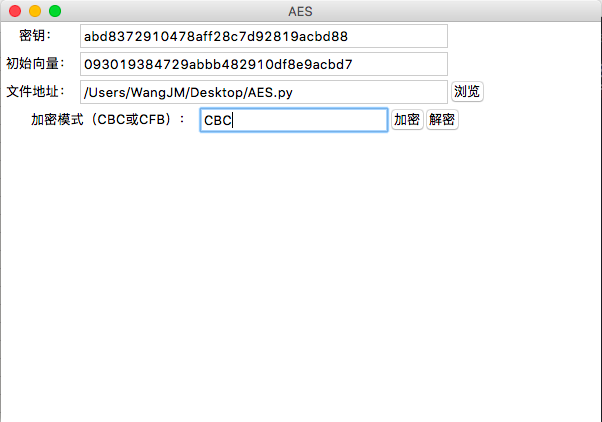
\includegraphics[height=8.44cm,width=12.04cm]{decrypt.png}
\caption{解密}
\label{decrypt}
\end{figure}
\begin{figure}[htbp]
\centering
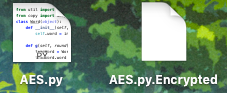
\includegraphics[height=4.65cm,width=11.35cm]{result.png}
\caption{加密后文件和解密出的文件}
\label{result}
\end{figure}
\newpage{}
\section{感想}
AES的实现使用面向对象的编程方式能大大简化操作,让逻辑变得非常清晰。本次实验对我的锻炼更多地来自于编程方面,因为AES算法本身并不复杂。我熟悉了python的GUI界面设计和面向对象的各种方法。然而python的运行速度给我带来了很大的困扰,其加密文件的大小只能限于几kb。这一方面是算法优化不足的问题,更大的还是语言问题。如果使用c++等编译型语言甚至是硬件语言,能大大加快速度。因此我并没有很纠结于速度的优化,而是更加重视实现本身。如果要让用python实现的AES算法去加密比较大批量的文件,实在有点勉为其难。

这次实验依然花了我很多时间,估计以后也将一直如此。无论这是好是坏,我只能接受然后面对。
\end{document}